\documentclass[a4paper,twoside]{article}

\usepackage{epsfig}
\usepackage{subfigure}
\usepackage{calc}
\usepackage{amssymb}
\usepackage{amstext}
\usepackage{amsmath}
\usepackage{amsthm}
\usepackage{multicol}
\usepackage{pslatex}
\usepackage{apalike}
\usepackage{SCITEPRESS}     % Please add other packages that you may need BEFORE the SCITEPRESS.sty package.

\usepackage{url}% http://ctan.org/pkg/url
\usepackage{flushend}

\subfigtopskip=0pt
\subfigcapskip=0pt
\subfigbottomskip=0pt

\begin{document}


\title{Enabling GPU Virtualization in Cloud Environments}
\author{\authorname{Sergio Iserte, Francisco J. Clemente-Castell\'o, Adri\'an Castell\'o,\\Rafael Mayo and Enrique S. Quintana-Ort\'i}
\affiliation{Department of Computer Science and Engineering\\Universitat Jaume I - Castell\'o de la Plana, Spain}
\email{\{siserte, fclement, adcastel, mayo, quintana\}@uji.es}}

\keywords{Cloud Computing, GPU Virtualization, AWS, Resource Management}

\abstract{The use of accelerators, such as graphics processing units (GPUs), to reduce the execution time of compute-intensive applications has become more popular during the past few years. 
These devices increment the computational power of a node thanks to its parallel architecture.
This trend has led cloud vendors, as Amazon Web Services, or middlewares such as OpenStack to add to their current facilities   
instances of virtual machines including GPUs. 
To fullfil these needs, the guest hosts must be equipped with GPUs which will be barely utilized if a non GPU-enabled Virtual Machine is running in the host.
The solution presented in this work is based on GPU virtualization and shareability in order to reach an equilibrium between service supply and applications' demand of accelerators. 
Hence, we propose to decouple real GPUs from the nodes by using the virtualization technology rCUDA. 
With this software configuration, GPUs can be accessed from any VM avoiding the need  
of having a physical GPUs in the guest host. 
Moreover, we study the viability of this approach by using a public cloud 
service configuration and develop a module for OpenStack middleware in order to 
add support for the virtualized devices and the logic to manage them. 
The results demonstrate this is a viable configuration which adds flexibility to the current and well-known 
cloud solutions. 
}

\onecolumn \maketitle \normalsize \vfill

\section{\uppercase{Introduction}}
\label{sec:introduction}
Nowadays, many cloud vendors have started offering virtual machines (VMs) with GPUs in order to provide
GPGPU computation services to users. A few relevant examples include 
Amazon Web Services (AWS)\footnote{\url{https://aws.amazon.com}}, 
Penguin Computing\footnote{\url{http://www.penguincomputing.com}}, 
Softlayer\footnote{\url{http://www.softlayer.com}} and 
Microsoft Azure\footnote{\url{https://azure.microsoft.com}}.
In the public scope, one of the most popular cloud vendors is AWS, that offers a wide range of preconfigured instances ready to be launched.
Alternatively, owning the propper infrastructure, a private cloud can be deployed using a specific middleware such as
Openstack\footnote{\url{https://www.openstack.org}} or Opennebula\footnote{\url{http://opennebula.org}}.

Unfortunately, sharing GPU resources among multiple VMs in cloud environments 
is not straightforward as is in a physical servers resulting into a low utilization rate.
On one hand, instances in public clouds are not easily customizable. 
On the other, in a private cloud, although the instances can be customized in many aspects, when referring to GPUs
the number of options is reduced.
Moreover, neither vendors nor tools are offer GPGPU wasting the opportunity of providing flexibility and boosty the utilization of GPU resources in both private or public clouds.

These devices were adopted with the release of the CUDA programming model for
NVIDIA GPUs~\cite{cuda65}, which includes both high- and low-level application programming interfaces (APIs)
to allow the use of NVIDIA devices as general-purpose
accelerators.
Following CUDA, OpenCL~\cite{opencl} appeared as an attempt
to offer a cross-vendor solution.

The current approach to assemble a cluster with accelerators consist in installing 
one or more of these devices in each compute node.
However, these configurations often present a low
utilization rate of the computational resources
 because of mismatches between the application's type of parallelism
and the accelerators' architecture.

Remote virtualization has been recently proposed to deal with the low-usage problem 
(e.g. {rCUDA}~\cite{tonithesis},
DS-CUDA~\cite{dscuda}, gVirtus~\cite{gvirtus}, vCUDA~\cite{vcuda}, VOCL~\cite{vocl}, and SnuCL~\cite{snucl}).

Roughtly speaking these virtualization frameworks 
enable cluster configurations with fewer GPUs than nodes.  The goal is that 
GPU-equipped nodes act as GPGPU (general-purpose GPU) servers, yielding a CUDA-sharing solution that potentially achieves
a higher overall GPU load in the system.

The main goals of this work are to study current cloud solutions from 
the point of view of HPC field and GPU usage, and to analyze and improve 
them by adding flexibility with GPU virtualization. In order to reach 
this goal, we select rCUDA, a virtualization tool that is possibly the more complete 
and up-to-date for NVIDIA GPUs.

The rest of the paper is structured as follows. 
In Section~\ref{sec:background} the technologies we introduce used in this work;
Section~\ref{sec:state} summarizes previous work in this field; 
Section~\ref{sec:motivation} states the motivation to carry out this work;
the effort to use AWS is explained in Section~\ref{sec:workingaws};
while the work with Openstack is described in Section~\ref{sec:gpgpuOS};
finally Section~\ref{sec:conclusions} summarizes the advances and Section~\ref{sec:future} proposes the next steps
 of this research.

\section{\uppercase{Background}}
\label{sec:background}
\subsection{The rCUDA Framework}
\label{sec:rcuda}
{rCUDA}~\cite{toniparco} is a middleware that enables transparent access
to any NVIDIA GPU device present in a cluster from all compute
nodes. The GPUs can be accessed and shared between nodes, and a single node can use all the graphic accelerators
as if they were local.
These features focus in attaining higher accelerator utilization rates in the overall system while simultaneously reducing
resource, space, and energy requirements~\cite{energy14}.
rCUDA is structured following a client-server distributed
architecture: the client middleware runs in the same cluster node where the application demanding GPGPU
acceleration services is executed, providing a transparent replacement for the
native CUDA libraries. Furthermore, the server middleware is executed in the
cluster nodes from which the actual GPUs provide the requested GPGPU service.
To support a concurrent scenario where GPUs are shared between
processes\slash nodes, {rCUDA} manages separate device contexts for
each client application.

The {rCUDA} 5.0 client exposes the same interface as the regular NVIDIA
CUDA 6.5 release~\cite{cuda65}, including the runtime and driver
APIs as well as other commonly used libraries such as cuBLAS, cuFFT, cuSparse or cuRand.
Therefore, applications are not aware of the fact that they are being executed
on top of a virtualization layer.
To deal with new GPU programming models, {rCUDA} has been recently extended to accommodate 
directive-based models such as OmpSS~\cite{repara15} and OpenACC~\cite{cluster15}.

The integration of remote GPGPU virtualization with global
resource schedulers such as SLURM~\cite{sbacpad14} completes this powerful
technology, making accelerator-enabled clusters more flexible and
energy-efficient.

\subsection{Amazon Web Services}
\label{sec:aws}
AWS~\cite{aws} is a public cloud computing provider, 
composed of several services, such as 
 cloud-based computation, storage and other functionality, 
that enables organizations and/or individuals to deploy
services and applications on an on-demand basis. 
These services replace local IT infrastructure for companies and provide agility and instant elasticity matching 
perfectly with their software requirements.

From the point of view of HPC, AWS offers high performance facilities via 
instances equipped with GPUs and high performance network interconnection, which 
are common resources leveraged in this research field.

\subsection{OpenStack}
\label{sec:openstack}

OpenStack~\cite{OpenStack} is a cloud operating system that provides Infrastructure as a Service (IaaS). 
It is able to control large pools of compute, storage, and networking resources throughout a 
datacenter. All these resources are managed through a dashboard or an API that gives administrators 
control while empowering their users to provision resources through a web interface
or a command-line interface.  
OpenStack supports most available hypervisors and handles provisioning 
and life-cycle management of VMs.
 
The OpenStack architecture offers flexibility to create a custom cloud, with no proprietary hardware
or software requirements and the ability to integrate with legacy systems and third party technologies. 

From the HPC perspective, OpenStack offers high performance configurations using
multiple supported hypervisors and different hardware architectures. Despite in OpenStack is possible to 
specify some extra parameters requesting special resources, like GPUs, choosing a host based on the existence
of a GPU is currently unsupported~\cite{OpenStackGPU}. 

\section{\uppercase{State-of-the-Art}}
\label{sec:state}
Our solutions to the defficiency exposed in the previous section is based on GPU virtualization, sharing resources in order
to attain a fair balance between supply and demand. 
While several efforst with the same goal have been made in the past, as exposed next, 
none of them is so ambitious as ours. 

The work in~\cite{younge2013enabling} allows the VM managed
by the hypervisor Xen to access the GPUs in the physical
node, with the implied limitations that a node cannot 
use more GPUs than those hosted in the machine, and idle GPUs can not be shared with other machines. The solution presented 
by gVirtus~\cite{giunta2010gpgpu} virtualizes GPUs and makes
them accessible for any VM in the cluster. However, this kind
of virtualization strongly depends on the hypervisor and, so
does its performance. Another similar solution is presented in gCloud~\cite{diab2013dynamic}. 
iWhile this solution is not yet integrated in a Cloud Computing Manager, its main
drawback is that the code of the applications must be modified
in order to be run in the virtual-GPU environment. A runtime component to provide abstraction
and sharing of GPUs is presented in~\cite{becchi2012virtual}, which allows scheduling policies 
to isolate and share GPUs in a cluster for a set of applications. 
The work introduced in~\cite{jungpgpu} is more mature, however,
it is only focussed on compute-intensive HPC applications. 

Our proposal goes further and, in addition to 
bringing solutions for all kind of HPC applications, it is aimed
to boost flexibility in the use of GPUs.

\section{\uppercase{Motivation}}
\label{sec:motivation}

Cloud computing and storage have gained wide appeal  
during the last years thanks to the easy set up 
process and the low IT invest. The services offered in the cloud are useful for companies and individuals 
that look for temporary access to the last technology without spending a 
huge amount of money. In general, the systems provided by cloud 
companies match with the those requested thanks to its flexibility.

Two different kinds of cloud approaches are currently available:
on one hand, public facilities, such as AWS or 
Microsoft Azure that allow users to chose a pre-configured system.   
On the other hand, institutions/companies 
are able to deploy their own cloud infrastructure by a software as OpenStack.  

In both cases, the power of current cloud facilities relies on the use 
of VMs which  
emulate a physical node with its own 
CPUs, storage, network interconnection, GPU and operating system (OS). 
However, providing a VM equipped with a GPU implies
that the guest host must be equipped with at least one GPU, and
once it has been assigned to an instance, no other VM can use
it. Therefore, the number of VMs that are allowed to use GPUs is 
limited by the number of the installed devices. This lack of 
flexibility is also present in the cluster configurations, where 
depending on the users' necessities, 
two approaches to introduce GPGPU computation can be identified:
the conservative option, features a lot of hosts with GPUs to 
ensure that is likely to satisfy all requests; in a
more daring approach, a reduced count of some GPU-enabled nodes is available, in the hope that a large burst of GPU requests 
 does not exhaust the cluster's resources.

The use of a virtualization technology such as {rCUDA} adds 
the desired flexibility because this software detaches the GPUs 
from the nodes where they are installed, allowing all nodes in a cluster
not only to use them as if they were local, but also to share them 
achieving a higher utilization rate and reducing the idle periods.
Thanks to the ``shareability'' introduced by {rCUDA}, all VMs in the cloud 
environment can leverage and share all GPUs installed in 
the physical nodes, removing past limitations. 

Our work focuses on AWS as a public 
solution, and on OpenStack software as a private cloud environment. 
In order to achieve our goal, these cloud facilities need to be provided with the {rCUDA} software. In addition, for OpenStack, a module for managing virtualized GPUs 
needs to be implemented.  



\section{\uppercase{Working with AWS}}
\label{sec:workingaws}
In this section, first of all, the current user-level features 
provided by the Amazon Web Services are explained and analyzed 
from the point of view of the GPU usage. 
Finally, the scenarios and experiments where virtualized GPUs are utilized are 
described and first results are showed.

\subsection{Current Features}
This subsection explains the most common features checked during 
the virtual machine creation step.

\subsubsection{Instances}

An instance is a pre-configured virtual machine focused on an 
specific target. Inside the large list of instances offered by AWS, 
we can find: general purpose (T2, M4 and M3); computer science optimized 
(C4 and C3); memory optimized (R3); storage optimized (I2 and D2) and 
GPU capable instances (G2). Each kind of instance has its own purpose and its 
own price. Moreover, each instance has different number of CPUs and network 
interconnection which can be: low, medium, high or 10Gb.

For this study, carried out in June 2015, we worked in the AWS availability zone US EAST (N. VIRGINIA). 
So, at that moment the instances used had the features presented in the Table~\ref{table:awsInstances}. 

\begin{table}[htb]
\renewcommand{\arraystretch}{1.3}
\caption{AWS available HPC instances.}
\label{table:awsInstances}
\tabcolsep=0.09cm
\begin{center}\begin{tabular}{cccccc}
Name & vCPUs & Memory & Network & GPUs & Price\\ \hline \hline
c3.2xlarge & 8 & 15 GiB & High & 0 & \$ 0.21\\ \hline
c3.8xlarge & 32 & 60 GiB & 10 Gb & 0 & \$ 1.68 \\ \hline
g2.2xlarge & 8 & 15 GiB & High & 1 & \$ 0.65\\ \hline
g2.8xlarge & 32 & 60 GiB & 10 Gb & 4 & \$ 2.6 \\ \hline
\end{tabular}\end{center}\end{table}

The selection of these concrete types have the aim of using C3 family instances, which are not equipped with GPUs, as client whereas the instances of the G2 family are acting as servers.   

\subsubsection{Networking}
As it is shown in the Table~\ref{table:awsInstances}, each instance has a different 
network and taking into account that the use of the bandwidth 
is critical when GPU virtualization is applied, a simple test to verify the 
real network bandwidth is needed.

\begin{table}[htb]
\renewcommand{\arraystretch}{1.3}
\caption{IPERF results between instances.}
\label{table:iperf}
\tabcolsep=0.24cm
\begin{center}\begin{tabular}{cccc}
Server & Client & Network & Bandwidth\\ \hline \hline
g2.8xlarge & c3.2xlarge & High & 1  Gb/s\\ \hline
g2.8xlarge & c3.8xlarge & 10Gb & 7.5  Gb/s\\ \hline
g2.8xlarge & g2.2xlarge & High & 1 Gb/s\\ \hline
g2.8xlarge & g2.8xlarge & 10Gb & 7.5  Gb/s\\ \hline
\end{tabular}\end{center}\end{table}

The IPERF\footnote{\url{http://iperf.fr/}} tool has been executed between the instances showed in 
the Table~\ref{table:iperf} in order to know the real bandwidth.
Therefore, we can assure that the nomenclature ``High'' used in the 
network column correspond to a 1~Gb interconnection network and the 10~Gb has 
a real bandwidth of 7.5~Gb/s.
Moreover, it looks like the instances equipped with a ``High'' interconnection network
are software-limited up to 1~Gb/s due to the theoretical and real bandwidth 
match perfectly. The gap between real and theoretical can be observed with 
the 10~Gb interconnection which reaches up to 7.5~Gb/s.


\subsubsection{GPUs}
As it has been said before, an instance is based on a VM which is running on a real node with its own virtualized components, so it is possible that AWS could use a virtualization framework to offer GPU services to all the instances.
Although, the {\tt nvidia-smi} command informs us that the GPUs installed are NVIDIA GRID K520, we need to verify that they are non-virtualized devices so, we have executed the NVIDIA SDK test called {\tt bandwidthtest}. 
As it is shown in the Table~\ref{table:bwt}, as the bandwidth achieved in this test is higher than the network bandwith, it reveals that it is an ad-hoc GPU. 
% \begin{table}[htb]
% \renewcommand{\arraystretch}{1.3}
% \caption{NVIDIA SDK {\tt bandwidthtest} execution transferring 32MB using pageable memory using local GPU.}
% \label{table:bwt}
% \tabcolsep=0.09cm
% \begin{center}\begin{tabular}{cccc}
% Name &  Data Movement & Network & Bandwidth \\ \hline \hline
% g2.2xlarge & Host to Device & High& 3,004 MB/s \\ \hline
% g2.2xlarge & Device to Host & High& 2,809 MB/s\\ \hline
% g2.8xlarge & Host to Device & 10 Gb& 2,814 MB/s\\ \hline
% g2.8xlarge & Device to Host & 10 Gb& 3,182 MB/s\\ \hline
% \end{tabular}\end{center}\end{table}

\begin{table}[htb]
\renewcommand{\arraystretch}{1.3}
\caption{NVIDIA SDK {\tt bandwidthtest} execution transferring 32MB using pageable memory using local GPU.}
\label{table:bwt}
\tabcolsep=0.09cm
\begin{center}\begin{tabular}{ccc}
Name &  Data Movement & Bandwidth \\ \hline \hline
g2.2xlarge & Host to Device & 3,004 MB/s \\ \hline
g2.2xlarge & Device to Host & 2,809 MB/s\\ \hline
g2.8xlarge & Host to Device & 2,814 MB/s\\ \hline
g2.8xlarge & Device to Host & 3,182 MB/s\\ \hline
\end{tabular}\end{center}\end{table}

\subsection{Testbed Scenarios}
In this section, the different client-server configurations 
are explained. All the scenarios are based on the maximum number of instances 
that a user can freely select without submitting a formal request. 
In particular, the maximum number of ``g2.2xlarge'' is 5 and 2 for the ``g2.8xlarge'' instances.

All the instances deployed operate the RHEL 7.1 64 bit system and the version 6.5 of CUDA. 

\begin{itemize}
\item Scenario A (Figure~\ref{subfig:aws1}) shows the most common 
and used hardware configuration in real clusters, where each node is 
populated with one GPU. Here, a simple node is able to use up to 5 GPUs 
using the ``High'' network. 

\item Scenario B (Figure~\ref{subfig:aws2}) is composed by 2 server nodes equipped 
with 4 GPUs each one and a client that does not have any GPU. This scenario is using 
a 10Gb network and the client is able to execute application using up to 8 GPUs.

\item Scenario C (Figure~\ref{subfig:aws3}) joins both scenarios A and B. So a 
single client, using a 1Gb network interconnection, has 13 GPUs that can be used as if they were locally installed.
\end{itemize}

\begin{figure*}[ht]
\centering
\subfigure[5 remote GPUs over 1GbE.]{%
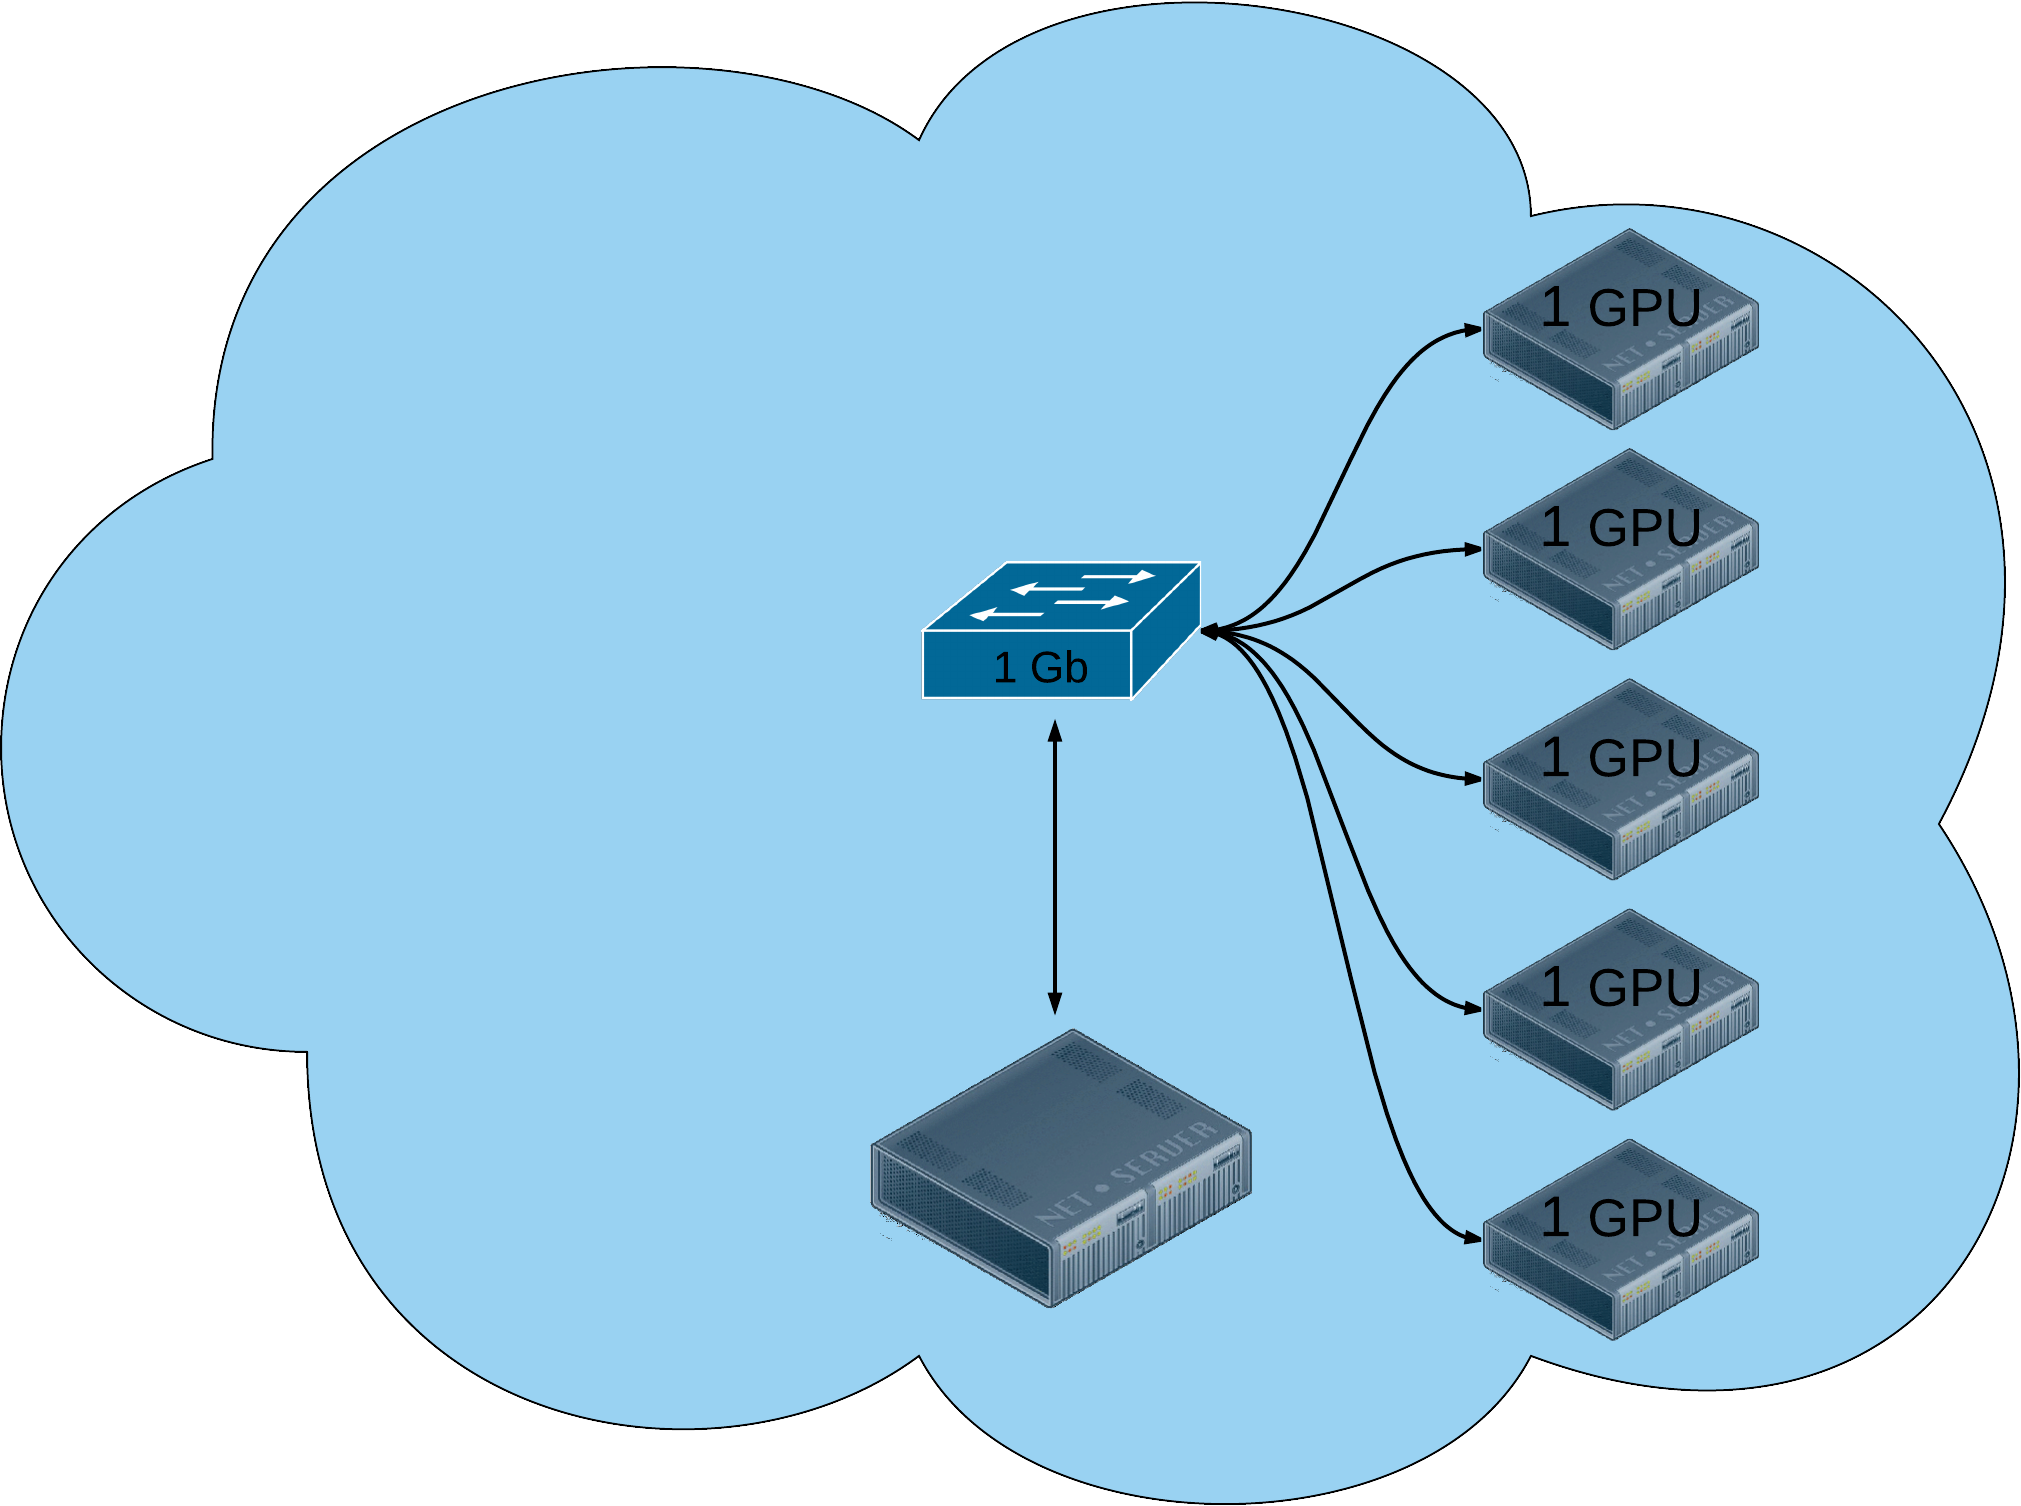
\includegraphics[width=0.31\linewidth]{images/aws3.png}
\label{subfig:aws1}}
\quad
\subfigure[8 remote GPUs over 10GbE.]{%
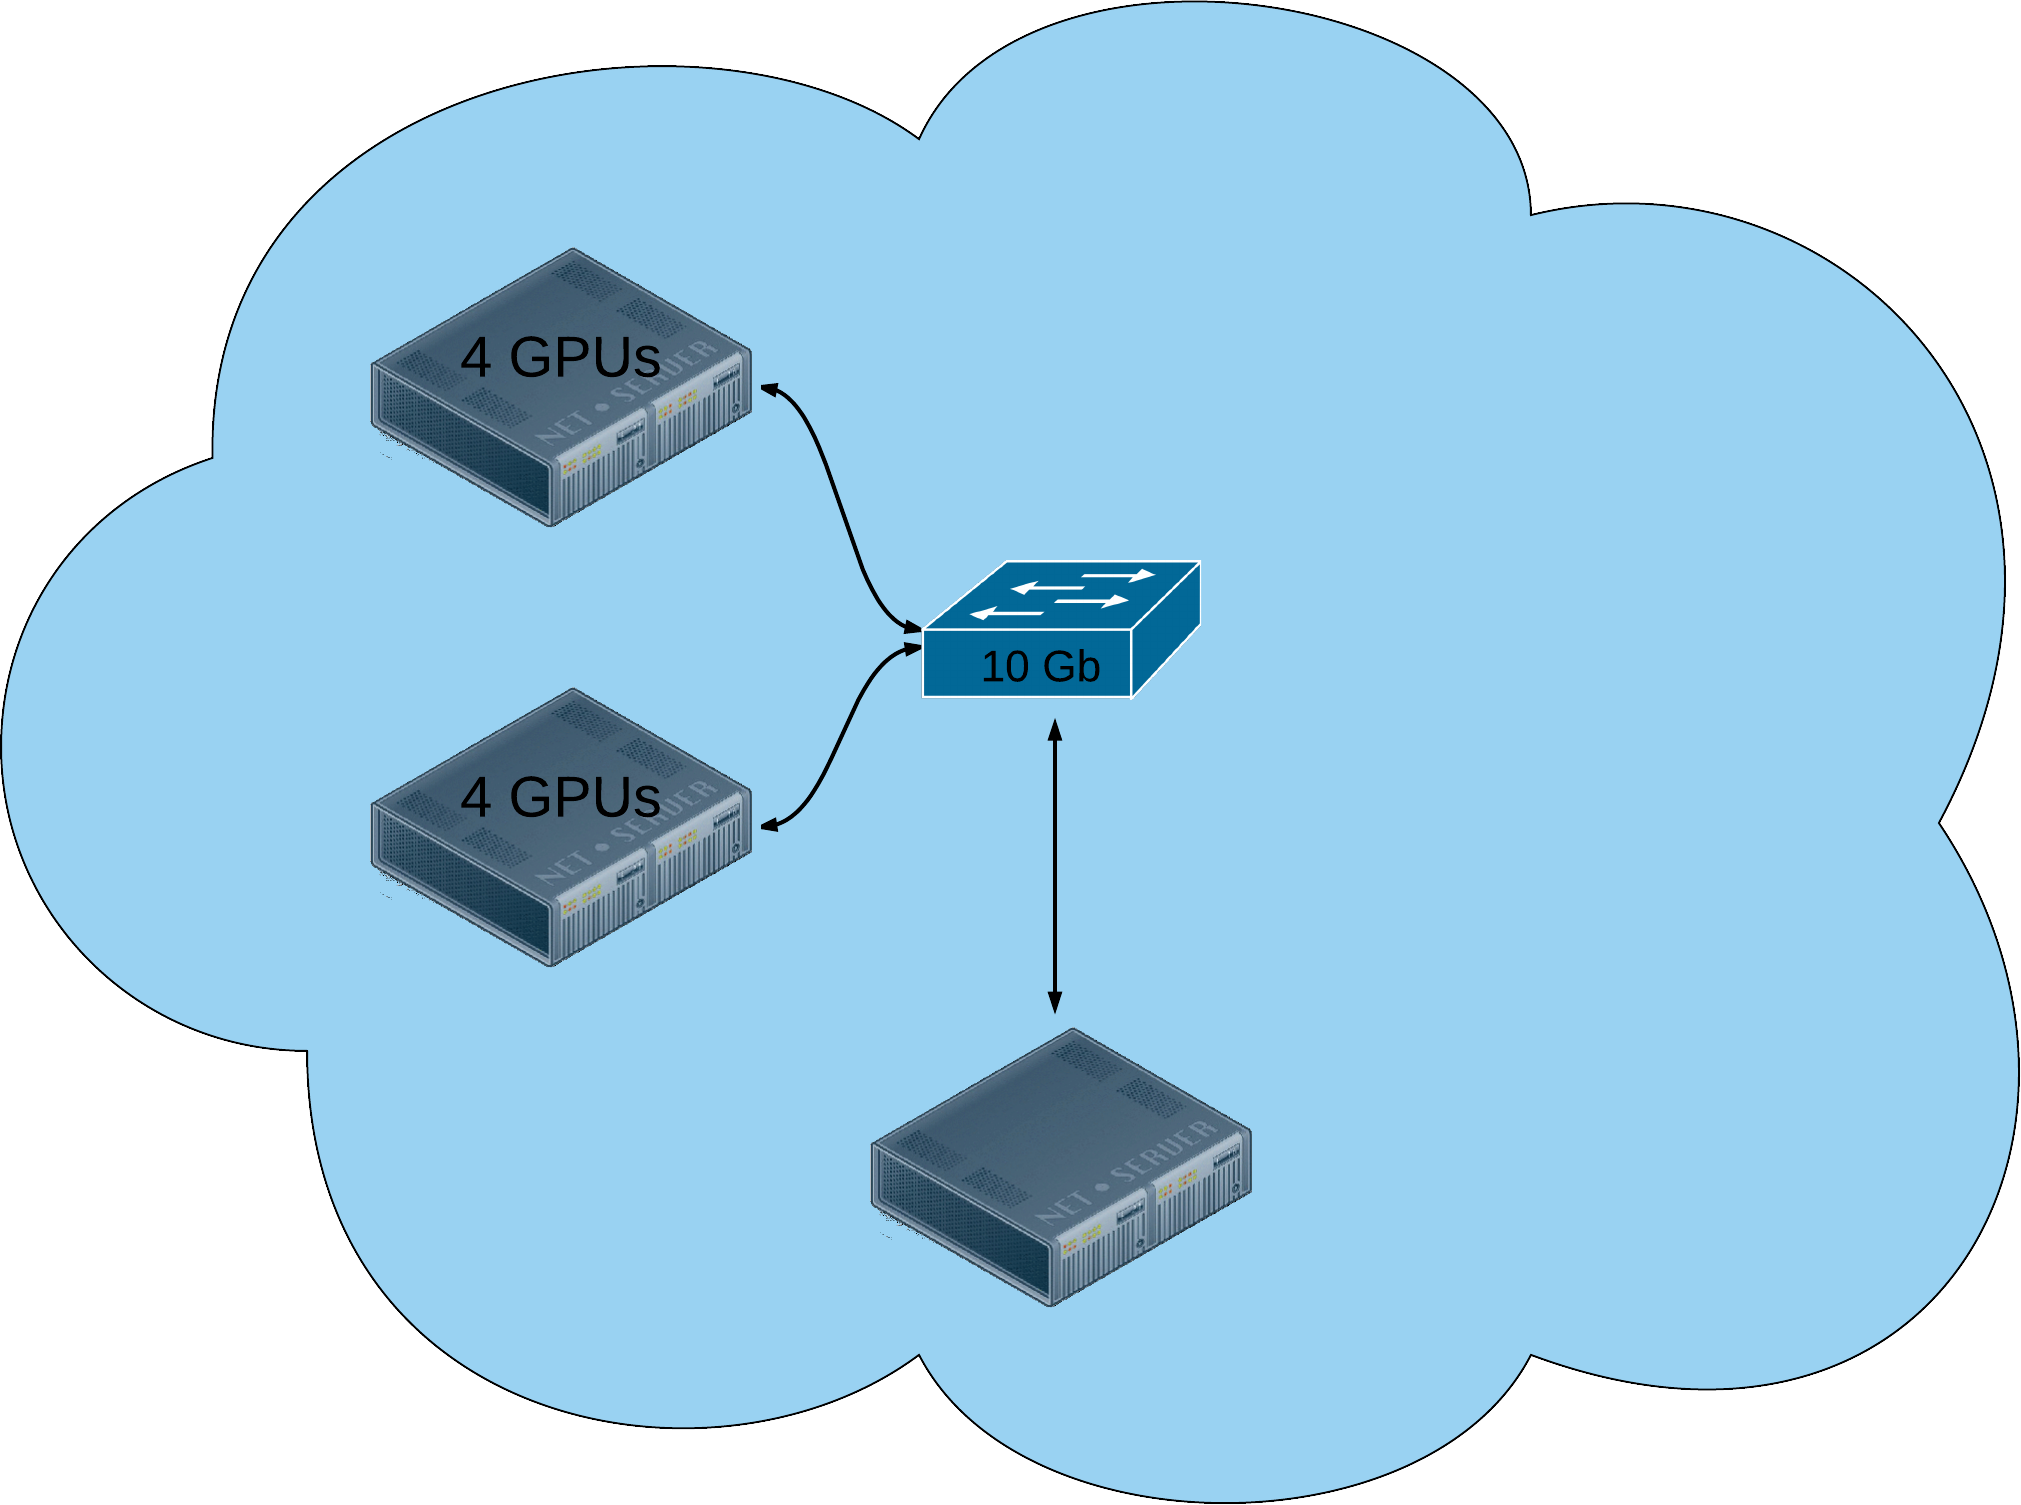
\includegraphics[width=0.31\linewidth]{images/aws2.png}
\label{subfig:aws2}}
\subfigure[13 remote GPUs over 1GbE.]{%
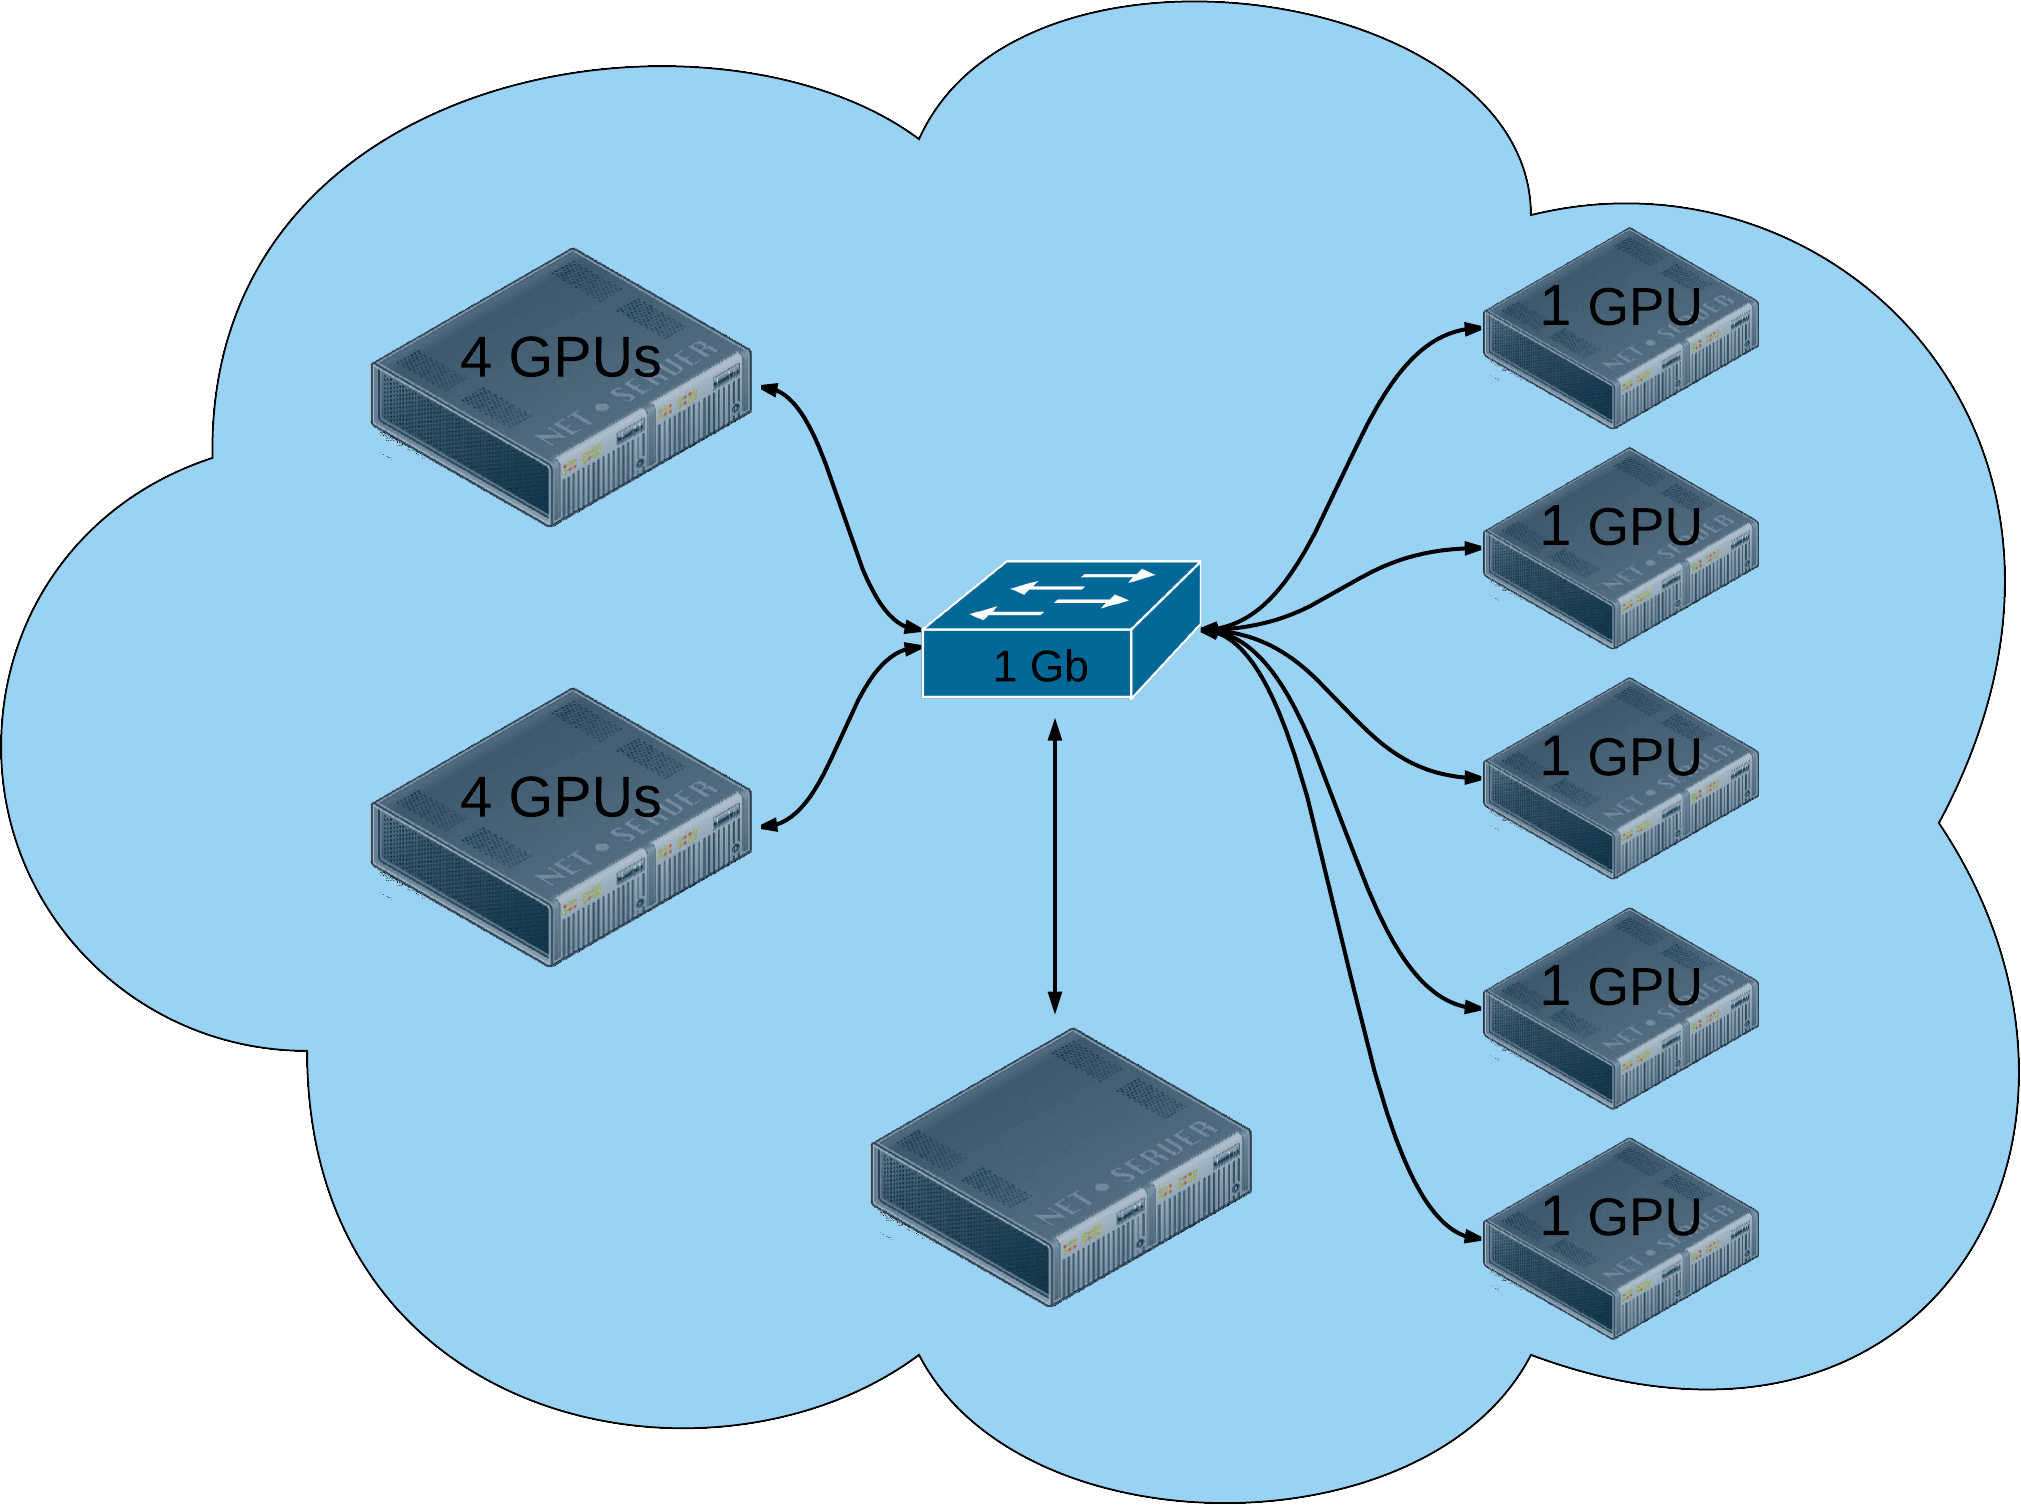
\includegraphics[width=0.31\linewidth]{images/aws1.png}
\label{subfig:aws3}}
\caption{Different configurations where an AWS instance acting as a client is using several remote GPUs.}
\label{fig:aws}
\end{figure*}

Once the scenarios are configured from the point of view of hardware, 
the {rCUDA} software needs to be installed in order to add 
the required flexibility to the system. So, the {rCUDA} server is 
executed in the server nodes and the {rCUDA} libraries are installed 
in the node that is acting as a client.

Moreover, with the aim to know the expected network bandwidth using 
a remote GPU, we have executed again the NVIDIA {\tt bandwidthtest} sample.
The results observed in the Table~\ref{table:bwtrcuda} shows how the bandwidth achieved is limited 
by the network.

\begin{table}[htb]
\renewcommand{\arraystretch}{1.3}
\caption{NVIDIA SDK {\tt bandwidthtest} execution transferring 32MB using pageable memory using {rCUDA}.}
\label{table:bwtrcuda}
\tabcolsep=0.09cm
\begin{center}\begin{tabular}{cccc}
Scenario &  Data Movement & Network & Bandwidth \\ \hline \hline
A & Host to Device & High& 127 MB/s \\ \hline
A & Device to Host & High& 126 MB/s\\ \hline
B & Host to Device & 10 Gb& 858 MB/s\\ \hline
B & Device to Host & 10 Gb& 843 MB/s\\ \hline
\end{tabular}\end{center}\end{table}

\subsection{Experimental results}
In order to assess that GPU virtualization with AWS instances was working as expected, two applications were executed to analyze the results and their scalability.

The first of them was {\tt MonteCarloMultiGPU} from NVIDIA SDK, an application purely computational. 
It was launched with the default configuration ``scaling=weak'' which adjust the size of the problem depending on the number of accelerators.
The Figure~\ref{fig:mont-opt} depicts the options per second calculated by the application running on the scenarios of Figure~\ref{fig:aws} and on the instances with local GPUs. 
We have removed the results of the Scenario B for clarity ought to they are exactly the same that the obtained from Scenario C up to 8 GPUs. 
In other words, we could state that the results until the 8th GPU would correspond to the Scenario B and thereafter to the Scenario C.
Hence, in this particular case, rCUDA (using remote GPUs) is performing better than CUDA (with its local GPUs) due to rCUDA loads the libraries when its daemon starts.
However, even with rCUDA we can see differences in the results between booth scenarios. We determined that the Scenario A could increase the throughput because
unlike the other setups the GPUs are not sharing the PCI bus with other devices, as it happens in the 4-GPU instances.
% \begin{figure}[!t]
%   \centering
%   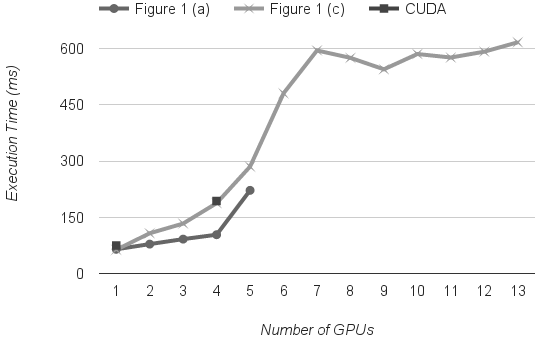
\includegraphics[width=\linewidth]{images/aws-mont2.png}
%   \caption{Montecarlo execution time}
%   \label{fig:mont-exe}
% \end{figure}
\begin{figure}[htb]
  \centering
  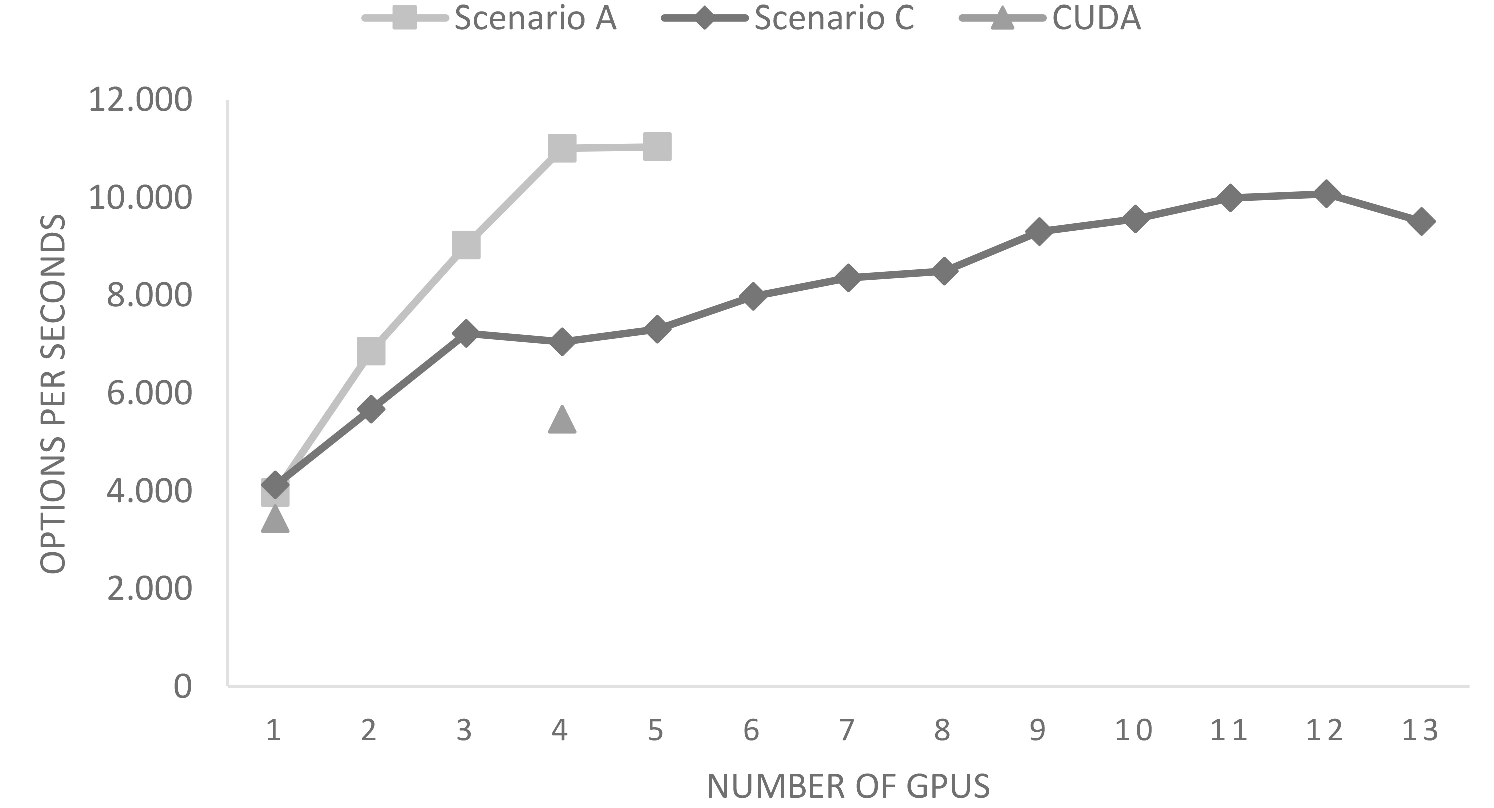
\includegraphics[width=\linewidth]{images/mont.pdf}
  \caption{NVIDIA SDK {\tt MonteCarloMultiGPU} execution using local and remote GPUs.}
  \label{fig:mont-opt}
\end{figure}

The other application, LAMMPS\footnote{\url{http://lammps.sandia.gov}}, is a classical molecular dynamics simulator that can be applied at the atomic, meso, or continuum scale. 
From the implementation perspective, this multi-process application employs at least one GPU to host its processes, but can benefit from the use of multiple GPUs.
The Subfigure~\ref{subfig:lammps1} shows that running this application using remote GPUs does not offer any advantage in front of original CUDA. 
Furthermore, for the execution on remote GPUs, a little difference between both networks can be appreciated, so, the ``High'' network performs worse than ``10 Gb'' network.
Thus, if we compare the results of a LAMMPS execution with a larger problem (see Subfigure~\ref{subfig:lammps2}), although CUDA continues performing better, the interesting point is the execution time on remote GPUs. 
They are almost the same even with different networks what means that the transfers are making the interconnection network the bottleneck, and enlarging the problem size
pays off the drawback of a slower network.

\begin{figure}[htb]
\centering
\subfigure[Run size = 100.]{%
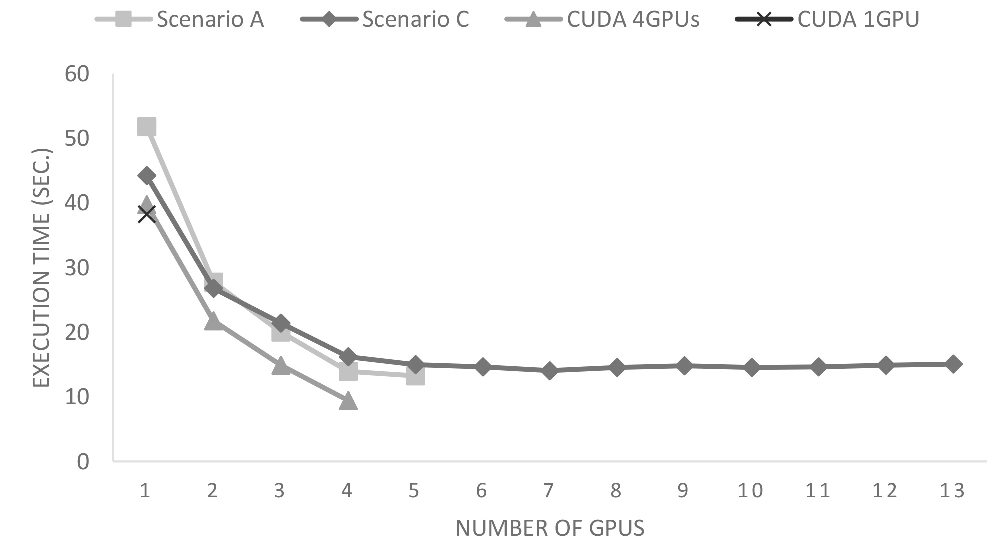
\includegraphics[width=\linewidth]{images/lammps1.pdf}
\label{subfig:lammps1}}
\quad
\subfigure[Run size = 2000.]{%
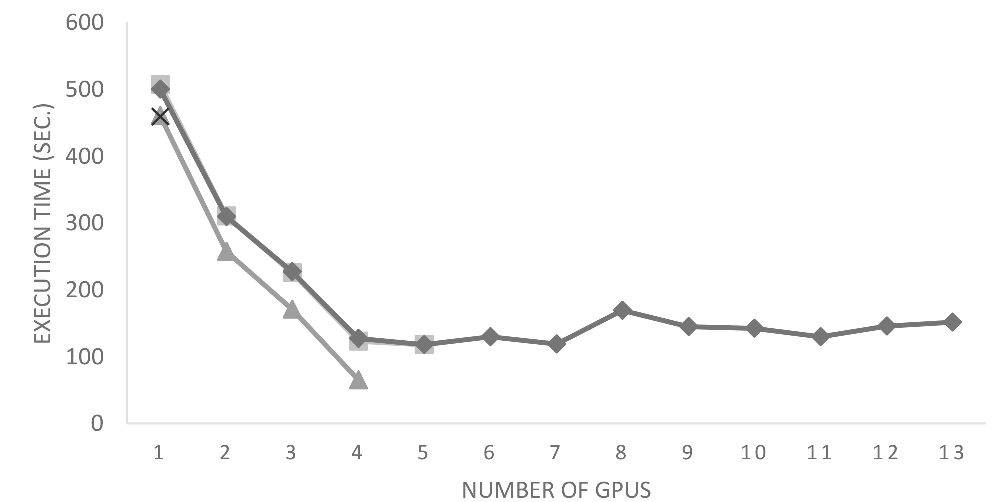
\includegraphics[width=\linewidth]{images/lammps2.pdf}
\label{subfig:lammps2}}
\caption{Execution time of LAMMPS.}
\label{fig:lammps}
\end{figure}

\subsection{Discussion}
Putting all together,  it is crystal clear that the AWS GPU-instances are not aimed to HPC because neither the network nor the accelerators are powerful enough to reach an appropriate performance
while running intensive parallel applications. 
Hence, AWS's target is more oriented to offer the service than to provide performance.
Also with the aim of plainly offering the service of GPGPU, AWS lacks in flexibility. 
AWS forces the user to choose between a basic instance with a GPU and a powerful instance with 4 GPUs.

Coming back to the Table~\ref{table:awsInstances} can be seen how not only the resources of the ``g2.8xlarge'' has been quadrupled, but also the cost per hour.
So, in the case of having other necessities (talking in terms of the instances type), with remotes GPUs we could attach an accelerator to any kind of instance.
Furthermore, reducing the budget in VM could be possible by customizing the resources of the available instances.
If needed, we could work on an instance of 2 GPUs for only \$ 1.3 by launching 2 ``g2.2xlarge'' and using remote GPUs. 
Avoiding to pay the double for features that we are not willing to use in ``g2.8xlarge''.

The last conclusion we will draw is related to GPU-shareability. 
As we deduced, AWS has GPU-capable physical machines reserved which could be idle until a GPU-instance request were made.
To have such an expensive accelerators in a standby state is counter-productive. So, it would make more sense if we had less devices, accessible from any machine, though.

\section{\uppercase{GPGPU Shared Service in OpenStack}}
\label{sec:gpgpuOS}
In this section all the work related to OpenStack that has been done is explained, from the development of an external module to handle remote GPUs to the physical setup and its testing.

\subsection{Managing remote GPUs with OpenStack}
The main idea is to move from the original OpenStack architecture (see Subfigure~\ref{subfig:os-orig})
 to a solution where a new shared service takes part into the architecture and it 
is responsible for all about GPU accelerators (see Subfigure~\ref{subfig:os-mod}).
This new service would bring more flexibility when managing GPUs and new working modes for GPGPU computation in the Cloud.
As it is shown in Figure~\ref{fig:internal}, we have altered the OpenStack original Dashboard with a new parser, 
which splits the HTTP query in order to make use of both, the GPGPU API for GPU-related operations, and the nova API for the rest of the computation. 
The new GPGPU Service has brought a new feature which brings more flexibility, apart from the regular idea of having GPUs in a VM, from now on, we can create ``GPU-pools''. 
A ``GPU-pool'' is a set of independent GPUs (logically disattached from the nodes) that can be assigned to one or more instances.

\begin{figure}[htb]
  \centering
  \subfigure[Version Icehouse]{
    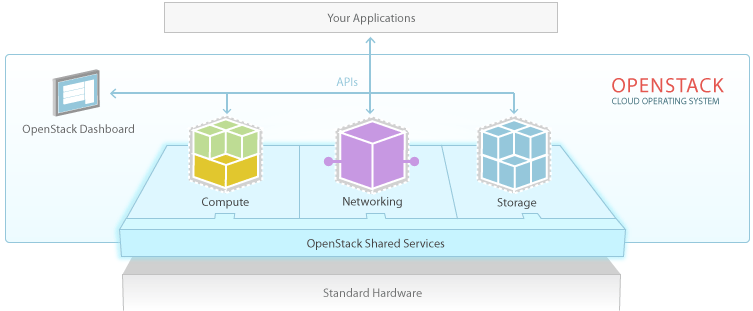
\includegraphics[width=\linewidth]{images/os-orig.png}
    \label{subfig:os-orig}
   }
   \quad
  \subfigure[With GPGPU developed module]{
    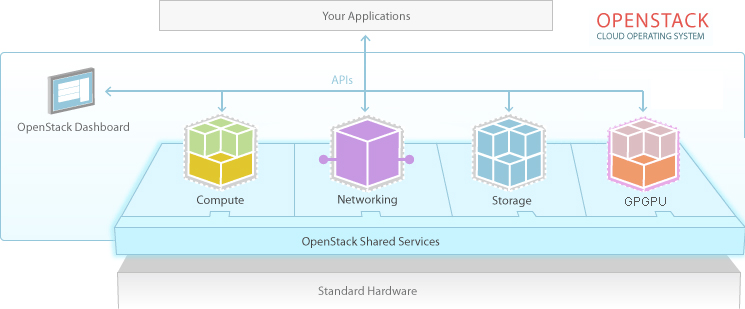
\includegraphics[width=\linewidth]{images/os1.jpg}
    \label{subfig:os-mod}
   }
  \caption{OpenStack Architecture}
  \label{fig:os}
\end{figure}

\begin{figure}[htb]
  \centering
  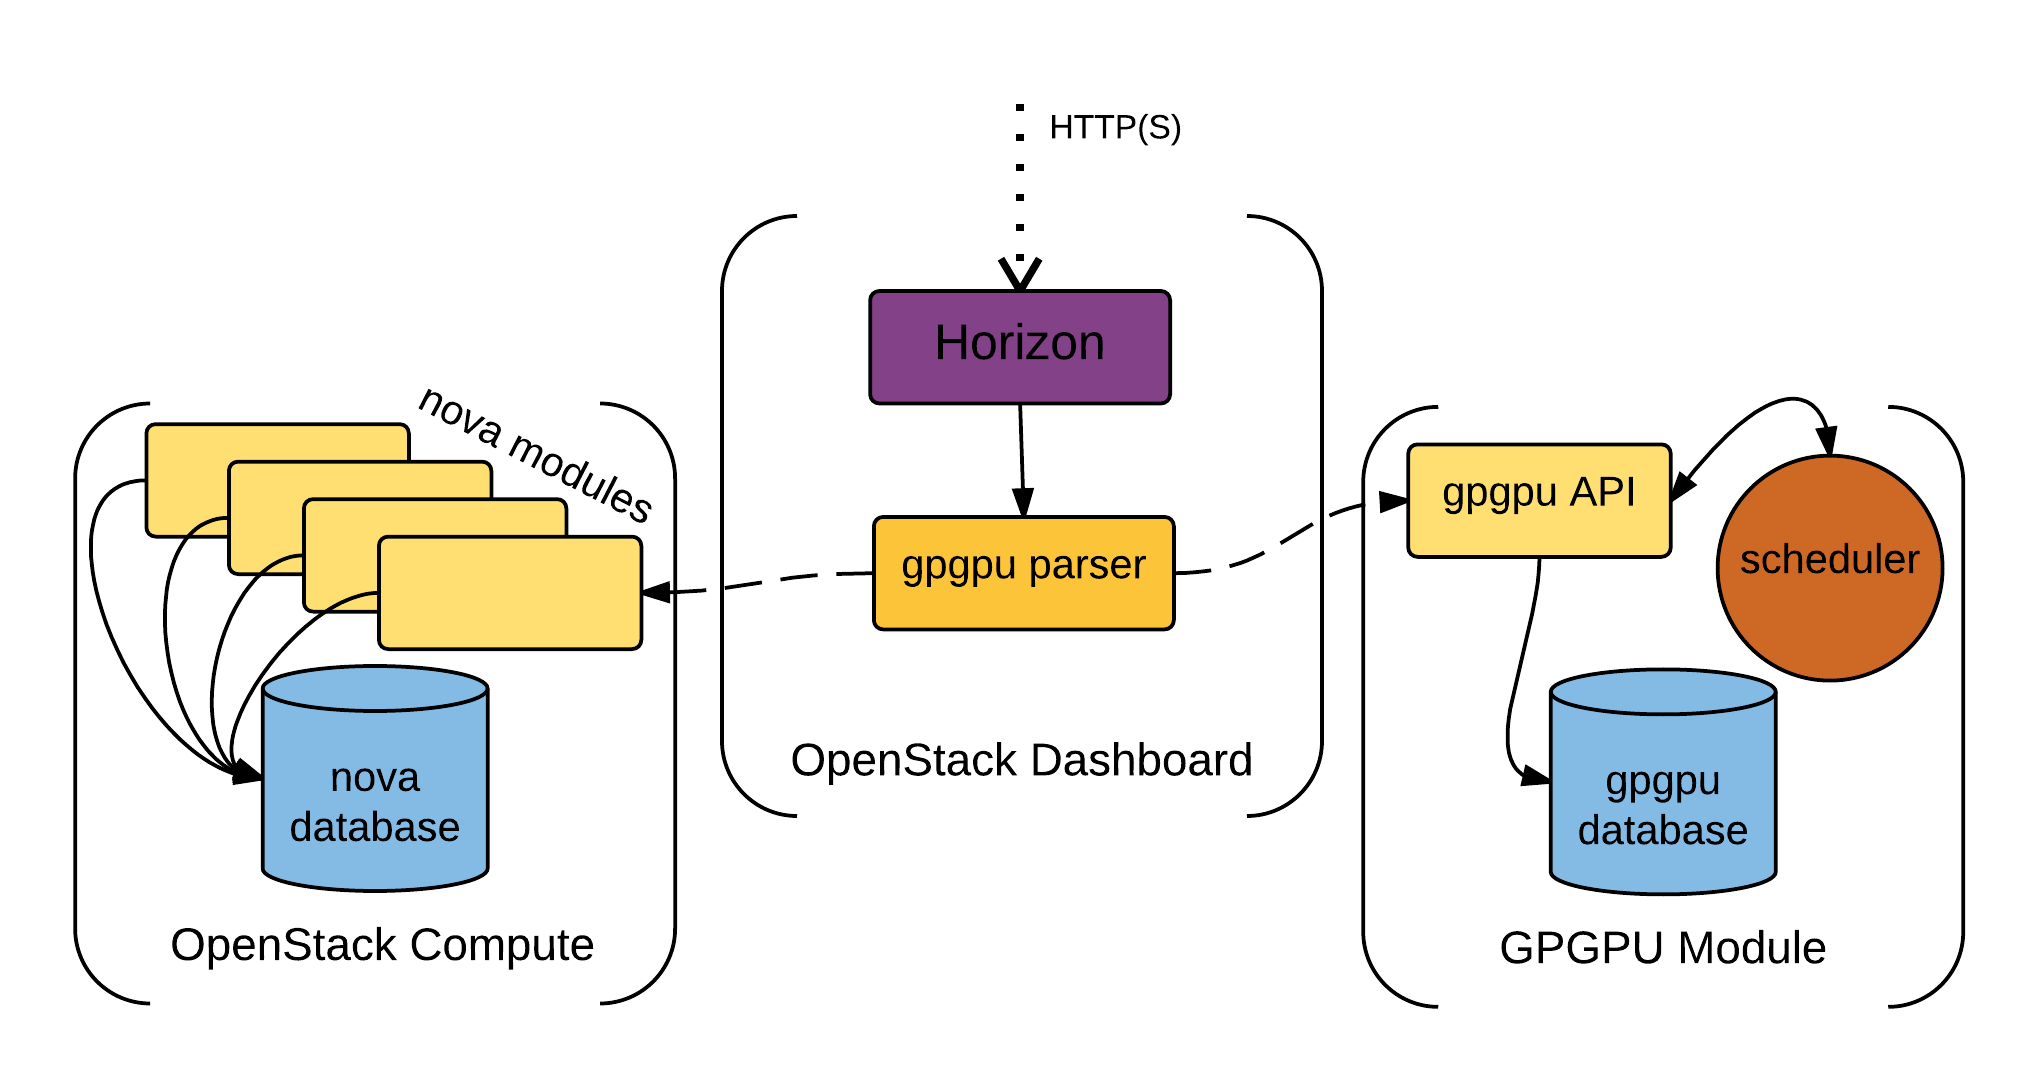
\includegraphics[width=\linewidth]{images/os2.png}
  \caption{Internal Communication among modules.}
  \label{fig:internal}
\end{figure}

Thanks to the modular approach of the GPGPU Service, the Nova Project has not been modified and the tool could be easily ported to other Cloud Computing solutions.

\subsection{Working Modes}
The developed module will allow the users to create any of the following scenarios (see Figure~\ref{fig2}). 
The users are given two configuration options to decide whether a physical GPU will be completely reserved for an instance (first column) or the instance will address a partition of the GPU as if it were a real device (second column).
We refer to this as the ``mode'' and the possible values for this parameter are: ``exclusive'' or ``shared''. 
Let us suppose to have 4 GPU devices in the cluster (no matter where they were hosted, neither if they were in the same server). 
A well illustrated example of those scenarios can be seen in the first row of the  Figure~\ref{fig2}.
So, while in ``exclusive'' mode the instance is monopolizing all the GPUs, in the ``shared'' mode the GPUs have been partitioned. 
As a result of halving the GPU memory of the accelerators, the instance will be able to work with up to 8 GPUs.

Moreover, the users are also responsible for deciding whether a GPU (or a pool) will be assigned to other instances. 
This behaviour is refereed as ``scope'' and it determines that a group of instances is logically connected to a pool of GPUs.
Working with ``public scope'' (second row of Figure~\ref{fig2}) means that the GPUs of a pool can be used simultaneously by all the instances linked to it.
Again, the GPU pool can be composed by ``exclusive'' or ``shared'' GPUs.

\begin{figure}[htb]
  \centering
  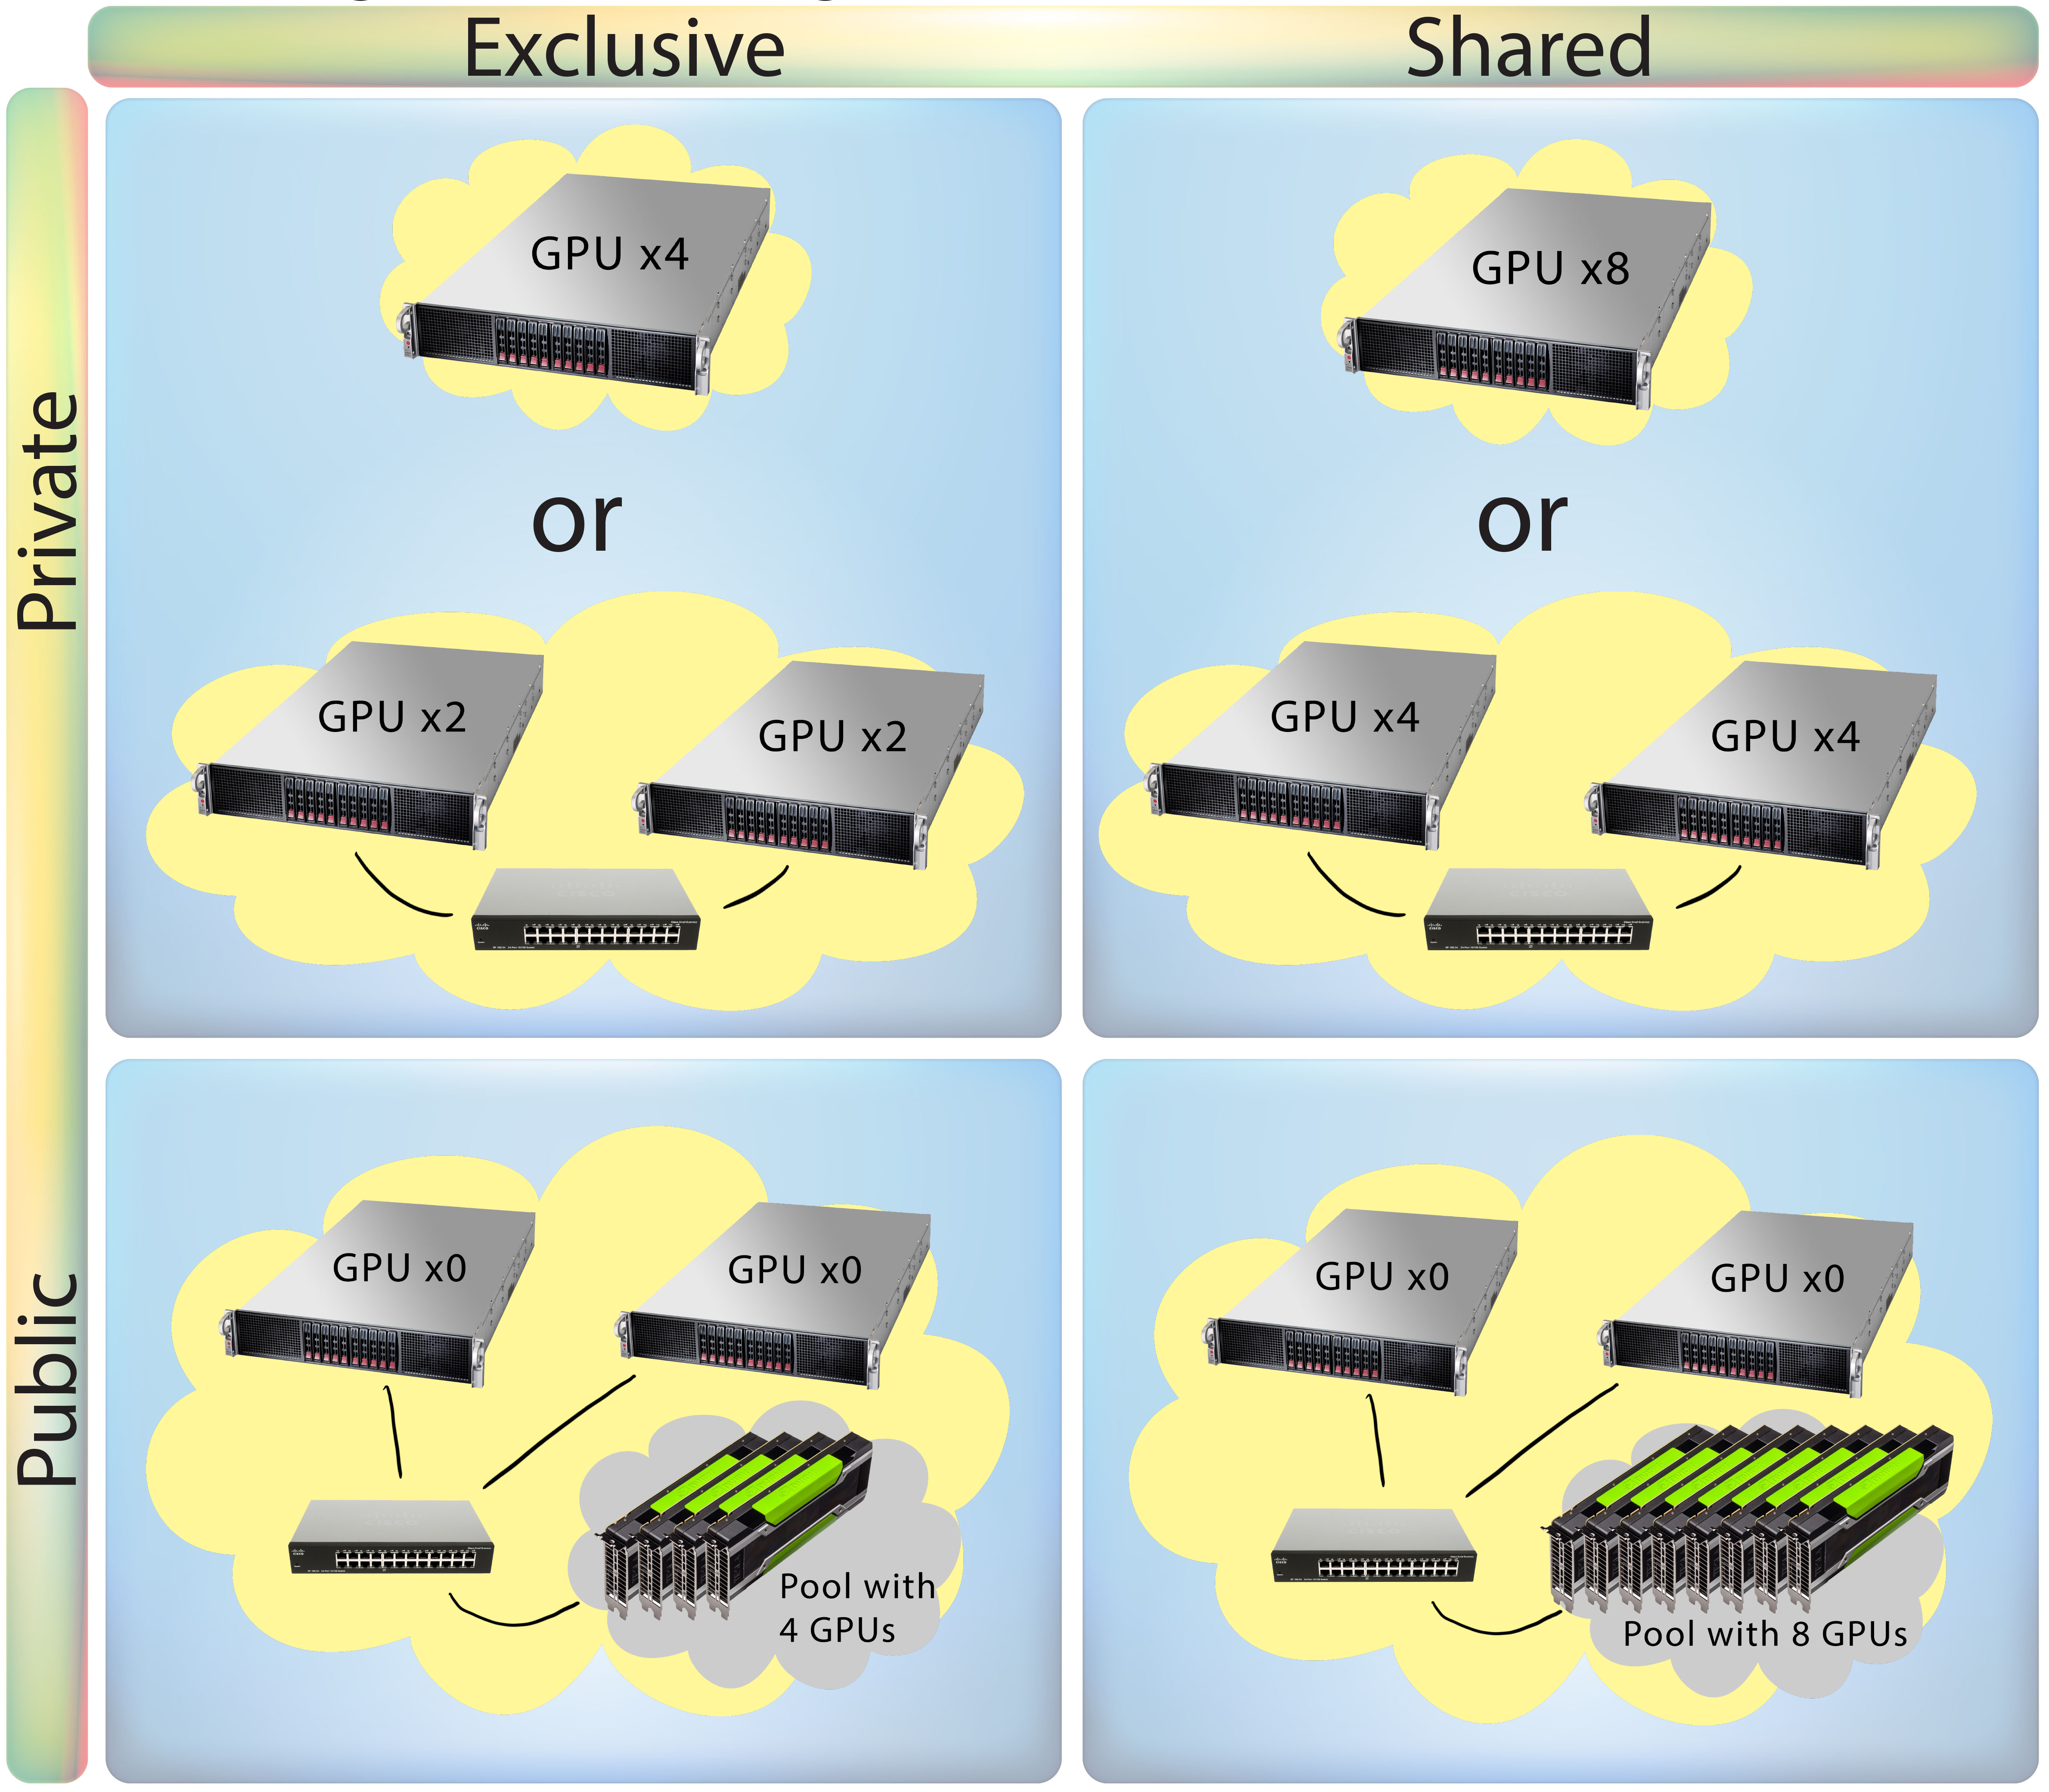
\includegraphics[width=.5\textwidth]{images/workingmodes.jpg}
  \caption{Examples of working modes.}
  \label{fig2}
\end{figure}

\subsection{User Interface}
Several modifications have been planned in the OpenStack Dashboard in order to deal with the new features.
First of all, the Instance Launch Panel should be provided with a new field, 
where the user could assign an existent GPU pool, create a new one or leave the instance without accelerators of this kind.
As soon as the option ``New GPU Pool'' is chosen, the proper fields for the pool configuration would appear (see Figure~\ref{fig:ui-launch}).
Furthermore, a new panel with the existent GPUs displays all the information related to GPUs (see Figure~\ref{fig:ui-rgpus}).

\begin{figure}[htb]
  \centering
  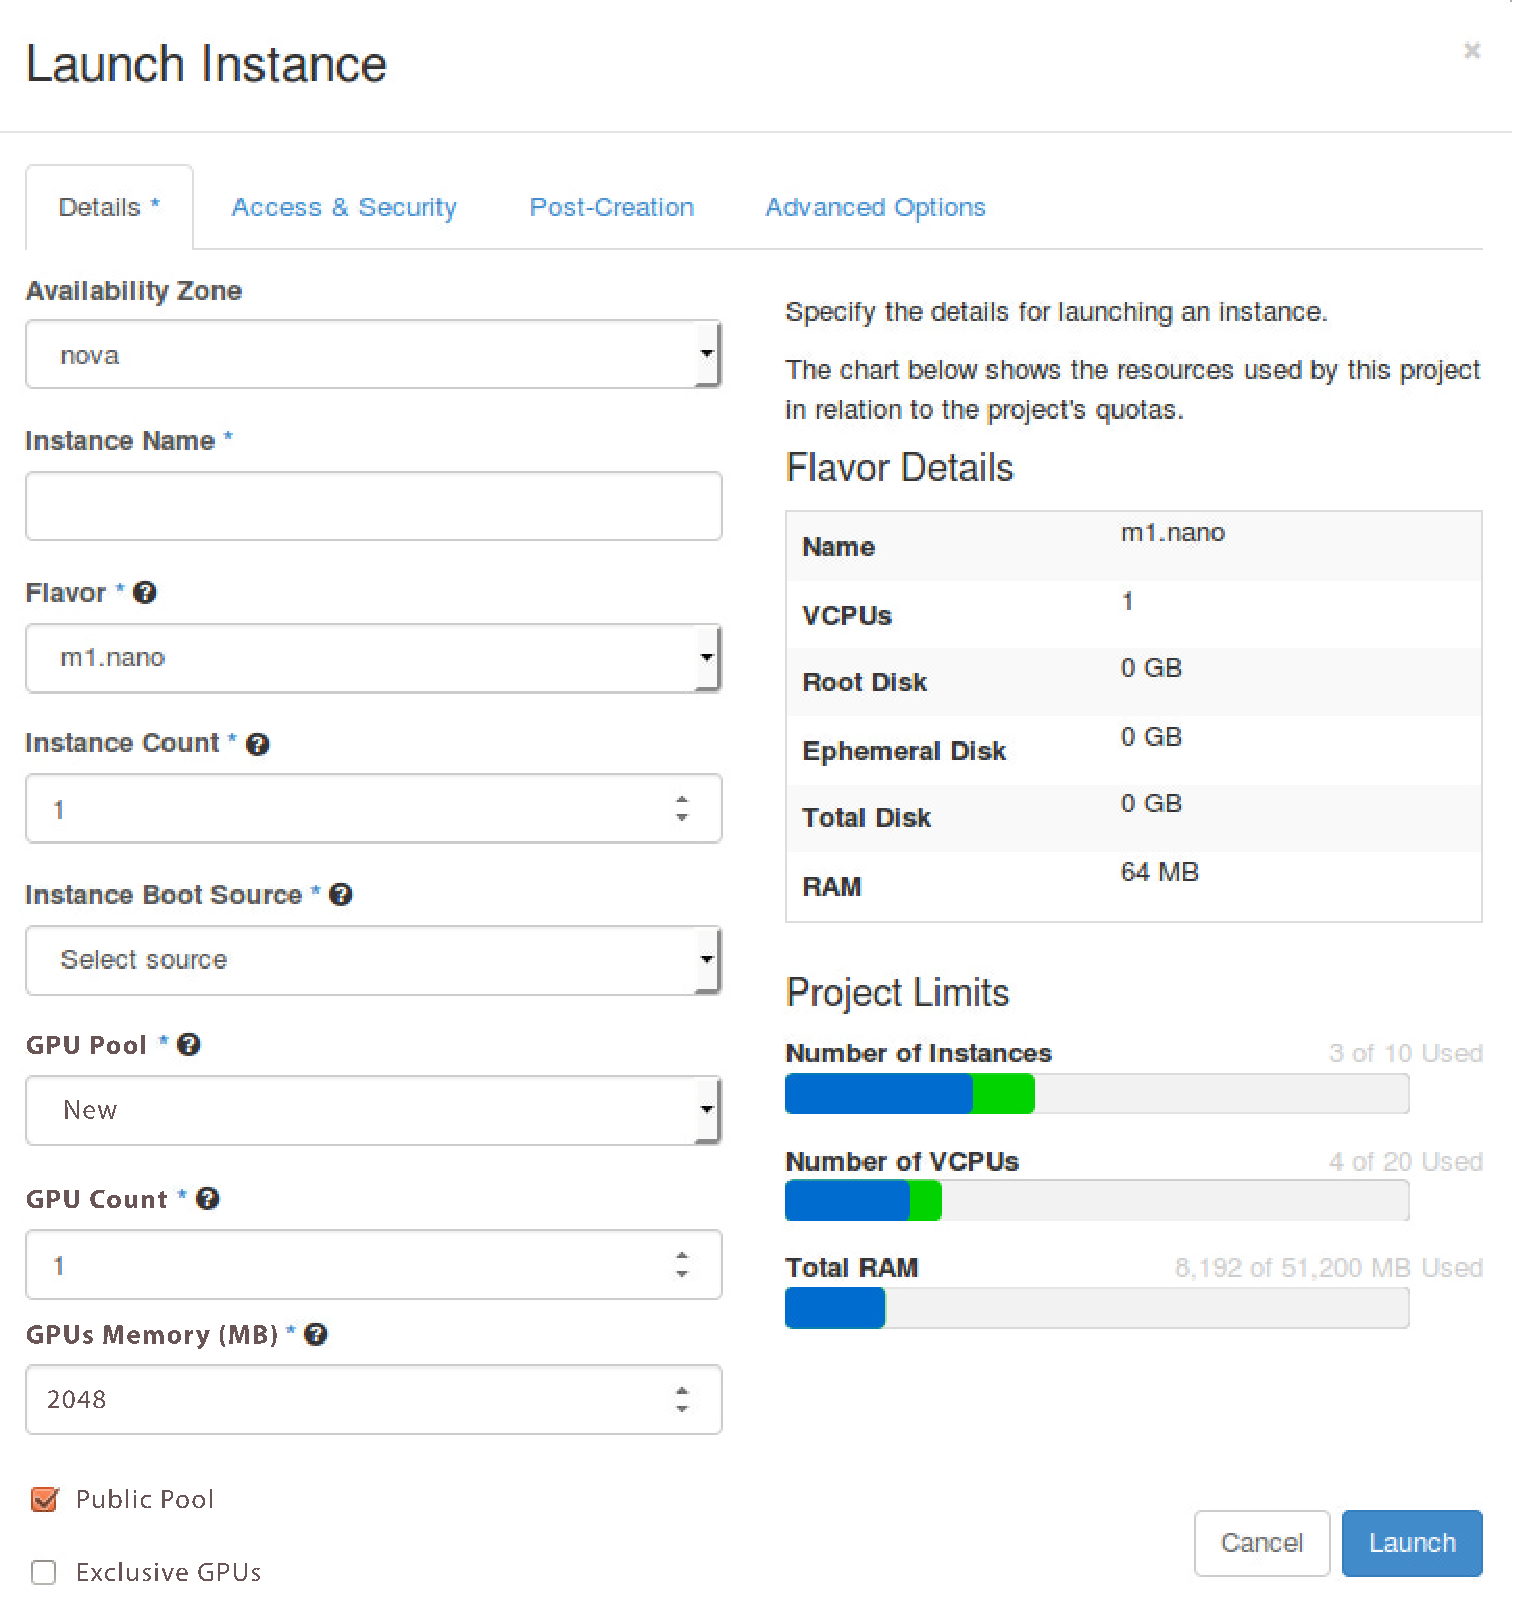
\includegraphics[width=\linewidth]{images/UI-launch.pdf}
  \caption{Launching Instances and assigning GPUs.}
  \label{fig:ui-launch}
\end{figure}
  
\begin{figure}[htb]
  \centering
  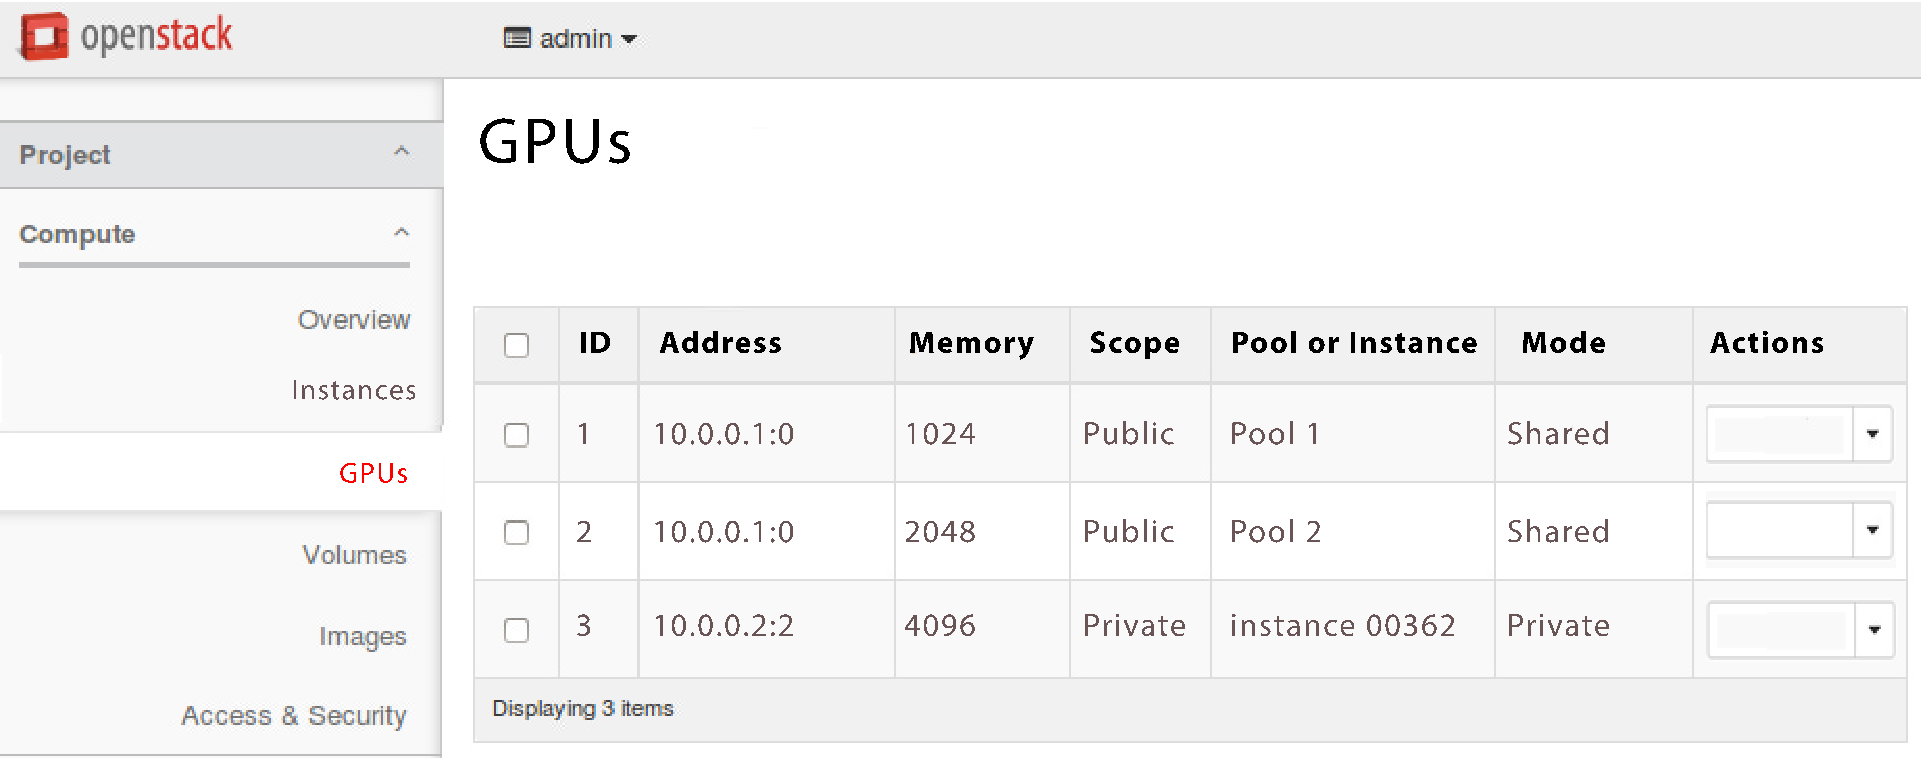
\includegraphics[width=\linewidth]{images/UI-rgpus.pdf}
  \caption{GPU Information Panel.}
  \label{fig:ui-rgpus}
\end{figure}

\subsection{Experimental Results}
The tests were executed on 2 sets of nodes interconnected through a 1Gb Ethernet network.

The first set, in charge of providing the cloud environment,
was composed of 3 nodes, each one equipped with an Intel Xeon E7420 quadcore processor at
2.13 GHz, and 16 Gbytes of DDR2 RAM memory at 667 MHz.
To deploy an infrastructure as a cloud service, we have used OpenStack Icehouse version and QEMU/KVM 0.12.1 as the hypervisors.
A fully-featured OpenStack deployment requires at least three nodes: one controller node that manages the compute nodes 
where the VMs are hosted, one network node that manages the logic
virtual network for the VMs, and one or more compute nodes that 
run the hypervisor and virtual machines.

The second set, composed by 4 nodes, were auxiliary servers with a Tesla C1060 GPU each one. 
Their system operates a Centos 6.6; and the GPUs use CUDA 6.5. 
The GPU virtualization support is based on rCUDA v5.0. 

We have designed 6 different set-ups which can be divided
into 2 groups: “Exclusive GPUs” and “Shared GPUs”. The
“Exclusive” mode will provide, at most, 4 accelerators. Whilst
the number of available GPU in “Shared” mode will depend
on the partition size. In this particular case, we have halved
the memory, so we can use up to 8 GPUs. For each group, we
have deployed virtual clusters of 1, 2 and 3 nodes where will
run the processes of the application. The instances are based
on the flavor “m1.medium” which determines VM of 2 cores
and 4096 MB of memory.

MCUDA-MEME~\cite{Liu2010} has been the application executed with
different configurations in order to test the set-ups. MCUDA-
MEME is an MPI application which is accelerated by GPUs.
Besides, each of its processes must have a GPU to not abort 
so, the number of GPUs will determine the number of processes that we can launch.

The Figure~\ref{fig3} shows and compares the execution time of
the application with different configurations over different setups. 
We have used up to 3 nodes to spread the processes and launched up to 8 processes (only 4 in exclusive mode), one for each remote GPU.
Firstly, we can state that the performance is higher with more than one node, because the traffic network is distributed among the nodes.
Secondly, the lowest execution time is obtained by both modes (exclusive and shared) when running their maximum number of processes with more than 1 node.
It could mean that it is not worthy to continue giving resources to the application to scale, because the performance growth rate is barely increasing.
Although, the time is lower sharing the GPUs the setup cannot take advantage of doubling the devices.

\begin{figure}[htb]
  \centering
  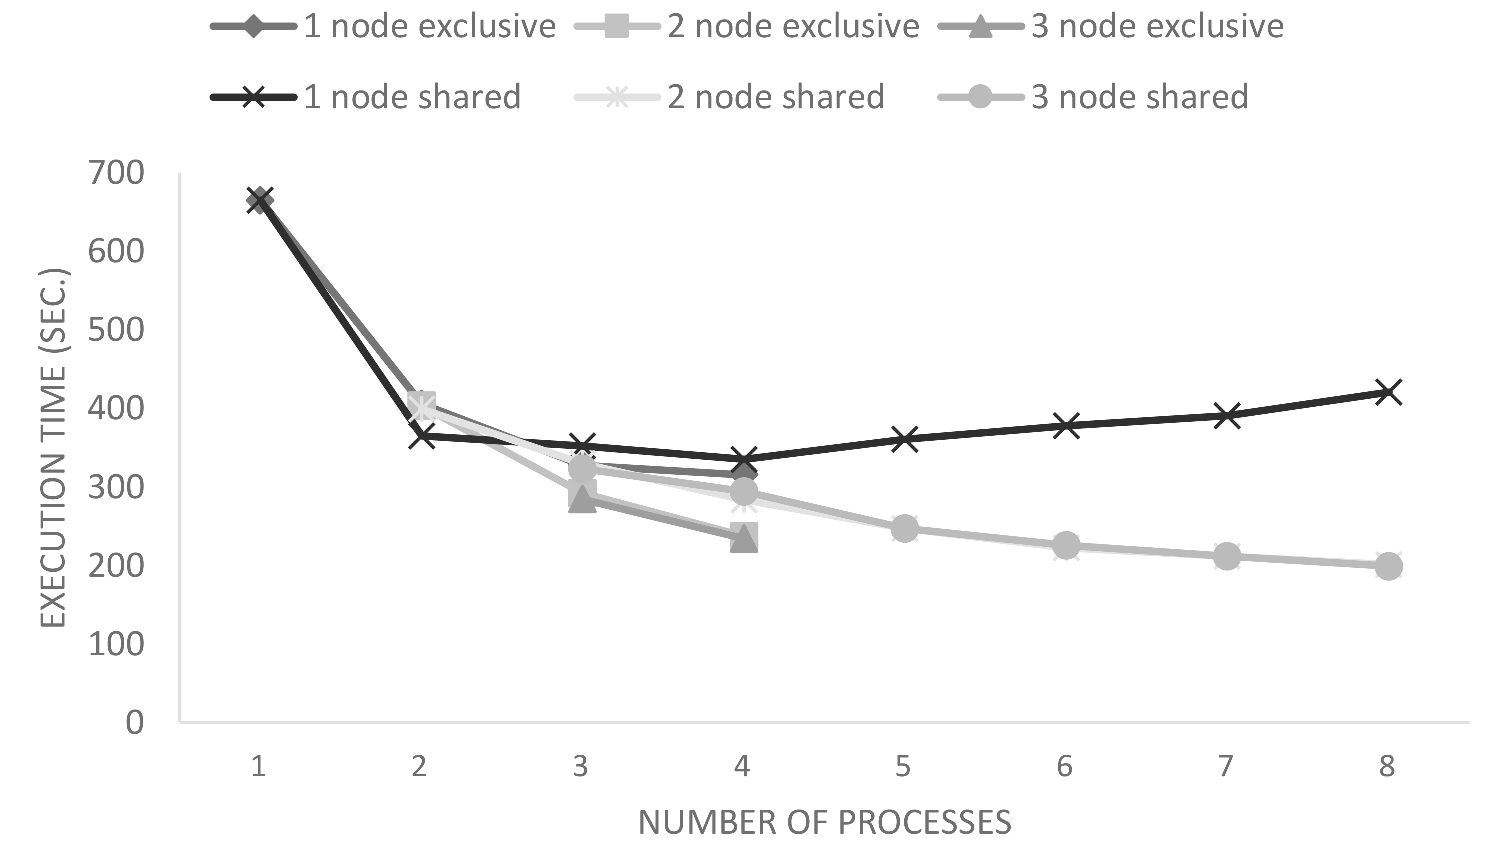
\includegraphics[width=\linewidth]{images/mcudameme-os.pdf}
  \caption{Scalability results of executing MCUDAMEME with a different number of MPI processes}
  \label{fig3}
\end{figure}

\subsection{Discussion}
Again, the networking issue is restricting the performance of our executions, but it has been discussed during virtually all the paper.
However, it is not a new topic and in~\cite{tonithesis} is explained that improving the network infrastructure could make the difference.

The most remarkable achievement is the wide range of possible configuration and the freedom that would have an administrator to set and reset a system to fit the 
user requirements. 

The requests of GPU-capable hosts in a completely transparent way for the user can be fulfilled with an small investment in infrastructure and in maintenance.
Energy can be saved, not only thanks to the remote access and the ability to emulate several GPUs from a real one, but also  by grouping the accelerators in a single machine (when possible) or turning down nodes when their GPUs are not necessary. 

\section{\uppercase{Conclusions}}
\label{sec:conclusions}
We have seen a thoroughly study of the possibilities offered by AWS in everything to do with GPUs. Its limitations drove us to deploy our own private cloud to have more flexibility when working with these accelerators.
So that, we have presented an upgrade for Openstack which easily permits to create GPU-instances and manage the physical GPUs to make more profit of them.

Leaving aside the performance of the executions which we knew in advance that would be poor due to the interconnection network features, we have created new operation modes. They have brought interesting new ways of using GPUs in situations where the simple fact of having accessing a GPU is more important than having a powerful GPU to boost the performance.

\section{\uppercase{Future work}}
\label{sec:future}
The first task that we should have keep in mind after this study is to upgrade the interconnection network to one more focused on HPC.
So that, porting the setup and the tests to an infrastructure with an Infiniband network would shed light on the viability of this kind of solutions for HPC.
The same thought, would guide us to try other Cloud vendors which more support for HPC.

Looking for real situations where the performance is not so important as the flexibility to provide more accelerators, 
would drive us to take the first steps through tools for easily deploying programming computer labs with the necessity for GPUs.

Other interesting approach would be to make the system energy-aware. 
Provided that a GPU could throw power information, a similar study based on the energy consumption could be done.

Finally, to bring in more strategies to decide where a remote GPUs is created and assigned to a physical device, would be an interesting task to carry out. 
With more scheduling policies the flexibility given by the GPGPU module for OpenStack would increase.

\section*{\uppercase{Acknowledgements}}
The authors would like to thank the IT members of the department Gustavo Edo and Vicente Roca for their help.

The researchers were supported by Universitat Jaume I research project (P11B2013-21), project
TIN2011-23283 and~FEDER.

\bibliographystyle{apalike}
{\small
\bibliography{paper}}


\end{document}
